\section{The Solenoid and the Steel Return Yoke}
\label{sec:solenoid}

The Compact Muon \emph{Solenoid} sports one of the world's most energetic solenoids which is paramount to the success of CMS.
Particles that exit the HCAL (subsec.~\ref{sec:hcal}) arrive at the cylindrical magnet which is 12.5 \meter in length, has a bore diameter of 6 \meter (6.3 \meter when cold), and generates a uniform 3.8 \tesla magnetic field parallel to the beam line.
To produce such a large and uniform magnetic field inside the approximately 360 $\meter^3$ volume (Fig.~\ref{fig:cms_magnetic_field}), an 18,000 amp current travels through the 4-layer, superconducting, NbTi coils.
This magnetic field is 100,000 $100,000$  $100000$ $100 000$ times stronger than Earth field at the surface, storing a massive 2.6 GJ of energy---approximately the kinetic energy of an Airbus A320 in flight.
The magnet has such a large stored-energy-to-cold-mass ratio (11.6 KJ/Kg) that it experiences a physical deformation of 0.15\% while energizing the field.
%%%%%%%%%%%%%%%%%%%%
\begin{figure}[pbth]
    \centering
    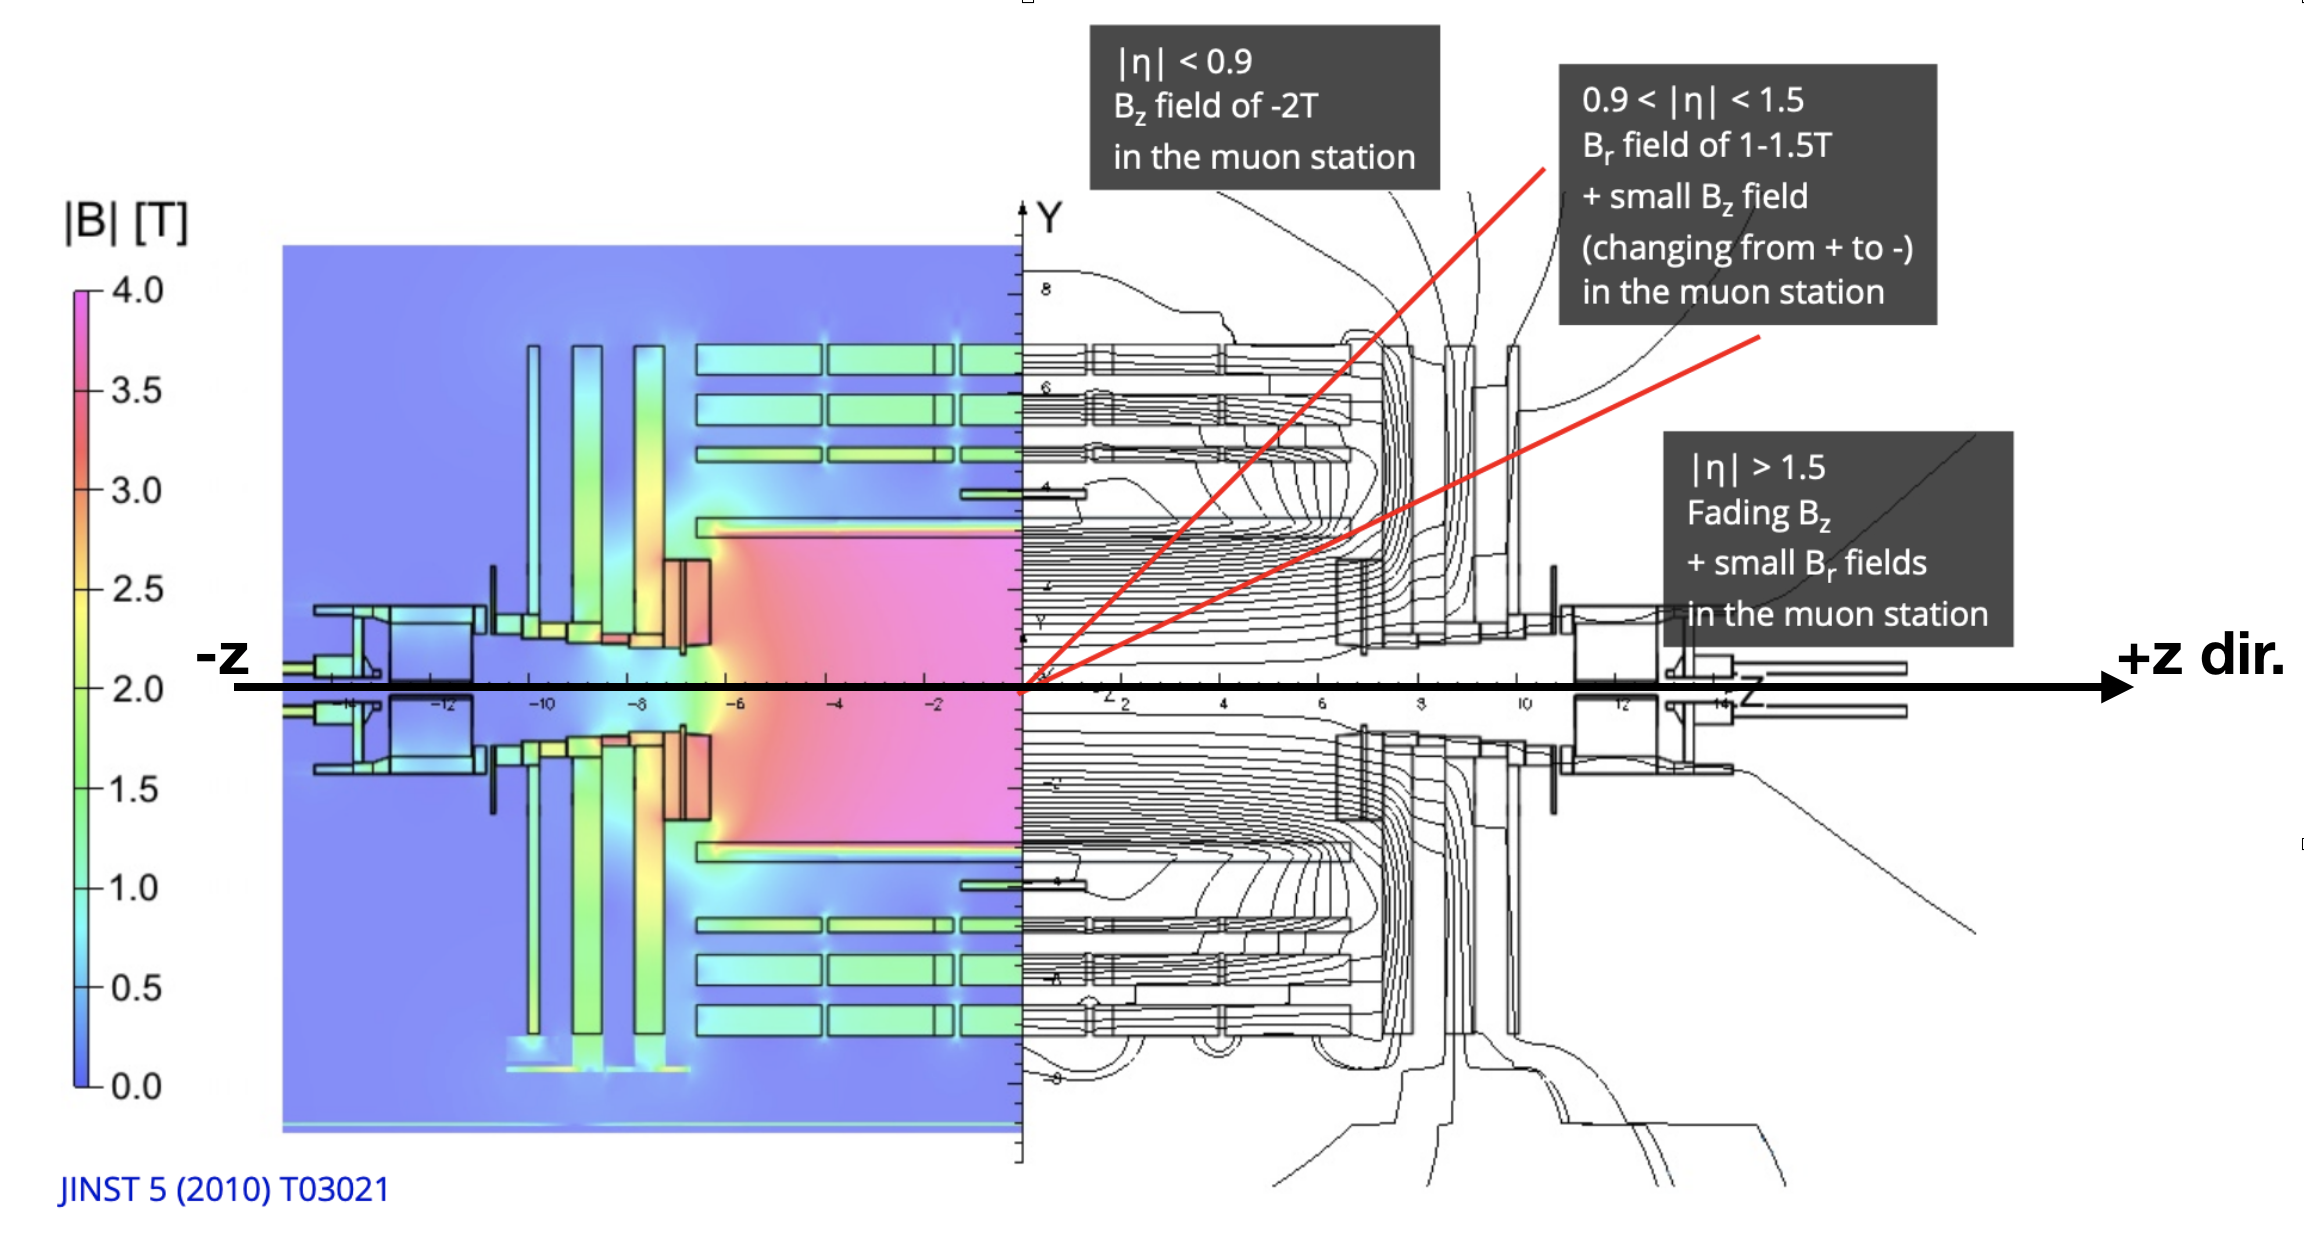
\includegraphics[width=15cm,height=15cm,keepaspectratio]{figures/cms/solenoid/CMS_longitudinal_view_magnetic_field.png}
        \caption{
        A longitudinal cross section of CMS showing the values of the magnetic field over the volume of CMS and various field lines. 
        The magnetic field reaches its maximum of 3.8 T in the center of the detector.}
        \label{fig:cms_magnetic_field}
    \end{figure}
    %%%%%%%%%%%%%%%%%%%%

As charged particles travel through any magnetic field, they experience a magnetic (Lorentz) force perpendicular to their direction of travel.
The Lorentz force $(\vec{F}_B)$ exerted on a particle with charge $q$ depends on the particle's velocity $(\vec{v})$ and the strength of the magnetic field $(\vec{B})$, given by
\begin{equation*}
    \vec{F}_B = q \vec{v} \times \vec{B}
\end{equation*}
Since the force is necessarily perpendicular to the velocity, the resulting trajectory is a helix.
Projecting the helix on the $x$-$y$ plane (since the magnetic field points in the $+z$ direction) allows the particle tracks to typically be separated from one another.
Each track has a corresponding radius of curvature $(R)$ which relates to its transverse momentum $(\pt)$ through
\begin{equation*}
    \pt = qBR.
\end{equation*}
The relative change in \pt (\ie the momentum resolution) is given by
\begin{equation}
    \frac{\delta \pt}{\pt} \propto \frac{\pt}{BL^2}.
\end{equation}

\textbf{Steel Return Yoke:} 
Most of the mass of CMS comes from the \emph{steel return yoke} which helps to redirect the magnetic field back on itself. 
The yoke system constitutes 10,000 tonnes, which is 89\% of the total mass of CMS.
It is comprised of 5 wheels and 2 endcaps
